\chapter{Introducción específica} % Main chapter title

\label{Chapter2}

%----------------------------------------------------------------------------------------
%	SECTION 2
%----------------------------------------------------------------------------------------
En este capítulo se presentan las tecnologías utilizadas en el desarrollo de este trabajo y se detallan sus características fundamentales de funcionamiento y sus especificaciones técnicas.

\section{Esquema general del sistema}

En la figura \ref{fig:diagBloques} se muestra el diagrama en bloques del sistema. Se pueden observar:

\begin{itemize}
	\item Red de sensores: recopila datos del entorno del invernadero.
	\item Nodo central: recibe datos de los sensores ESP-NOW y los envía al servidor a través de MQTT.
	\item Comunicación MQTT: facilita la transferencia de datos entre el módulo central y el servidor.
	\item Servidor IoT: almacena y procesa los datos recibidos de los sensores.
	\item PWA: permite el monitoreo y control del sistema en la red local.
	\item Red sensores y actuadores: recopilan datos y controlan dispositivos en el invernadero.
	\item Usuario remoto: accede a los datos recopilados a través del servidor IoT.
	\item Usuario local: accede a los datos a través de la PWA.
\end{itemize}

\begin{figure}[H]
\centering 
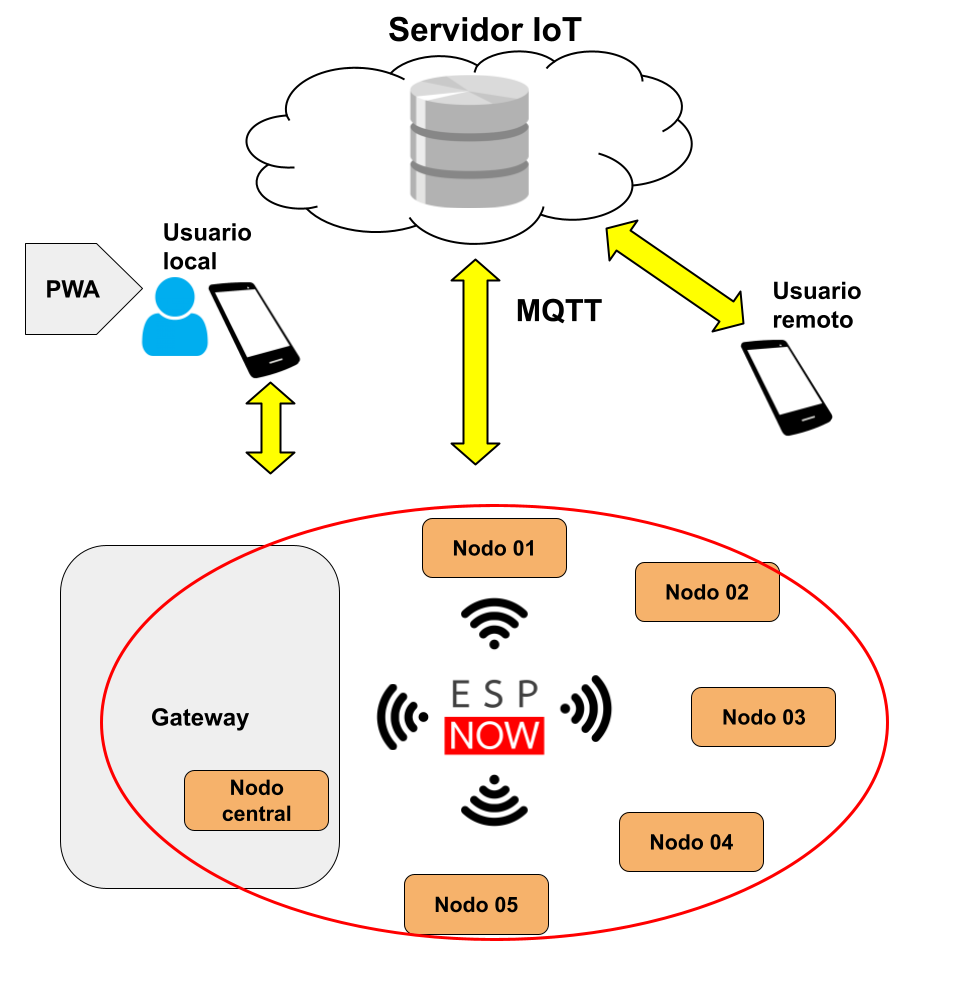
\includegraphics[width=.8\textwidth]{./Figures/Diagrama_bloques.png}
\caption{Diagrama en bloques del sistema.}
\label{fig:diagBloques}
\end{figure}



%----------------------------------------------------------------------------------------
\section{Tecnologías de hardware}

Los componentes de hardware fueron impuestos por la empresa Wentux, por lo que no se tuvo ninguna influencia en la selección del microcontrolador y los sensores.

\subsection{Microcontrolador}

Para los nodos sensores y el gateway del sistema, se utilizó la placa de desarrollo ESP32-C3 de Espressif Systems, un microcontrolador eficiente y versátil, ideal para aplicaciones de IoT. Cuenta con un núcleo RISC-V de 32 bits, que combina rendimiento y bajo consumo de energía, lo que optimiza la operación de los dispositivos en el sistema de monitoreo y gestión.
Este microcontrolador admite tanto Wi-Fi como Bluetooth 5 (LE) y ofrece múltiples opciones de conectividad inalámbrica. Además de estas tecnologías, soporta el protocolo ESP-NOW, una solución de comunicación inalámbrica propietaria de Espressif \citep{esp32c3}.

En la figura \ref{fig:esp32c3} se puede observar el módulo.

\begin{figure}[htpb]
    \centering
    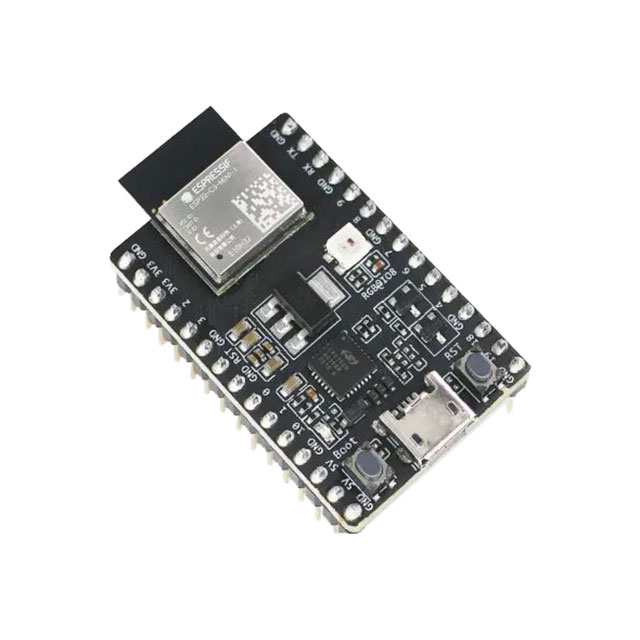
\includegraphics[width=.3\textwidth]{./Figures/esp32c3.png}
    \caption{Módulo ESP32-C3.}
    \label{fig:esp32c3}
\end{figure}

El ESP32-C3 también ofrece soporte para actualizaciones OTA (Over-the-Air), lo que facilita la actualización remota del firmware. Además, su amplio conjunto de interfaces de comunicación como UART, I2C, SPI, y ADC permite la integración con diversos sensores y actuadores, necesarios para la operación del sistema en el invernadero. 

La información completa sobre el microcontrolador y sus especificaciones técnicas está disponible en el sitio web oficial de Espressif \citep{docsesp32c3}.

\subsection{Sensores}

A continuación, se describen brevemente los sensores utilizados en el sistema.

\begin{itemize}
    \item Sensor LM35 \citep{sensor_lm35}: es un sensor de temperatura analógico que proporciona una salida de voltaje linealmente proporcional a la temperatura. Figura \ref{fig:lm35}.
\end{itemize}

\begin{figure}[H]
	\centering
	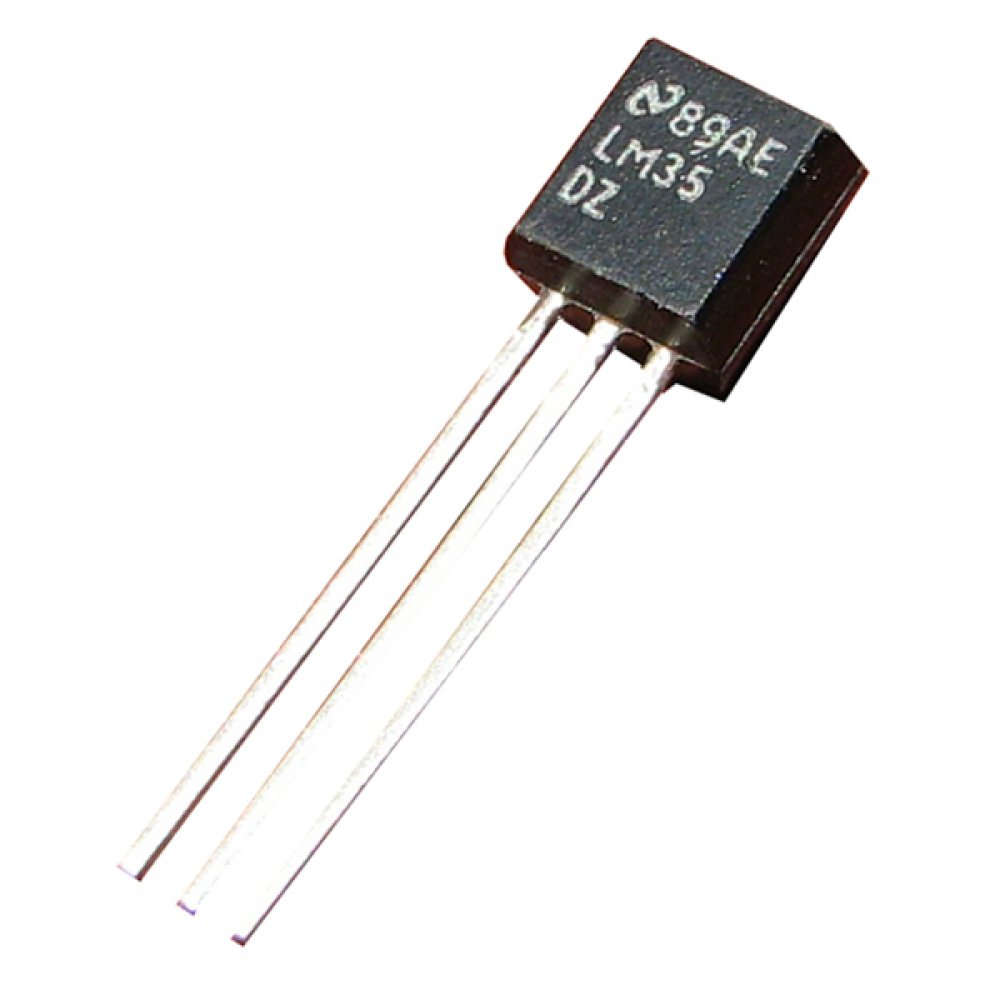
\includegraphics[width=.2\textwidth]{./Figures/sensor_lm35.png}
	\caption{Sensor LM35.}
	\label{fig:lm35}
\end{figure}

\begin{itemize}
	\item Sensor HTU21 \citep{sensor_htu21}: es un sensor digital de humedad relativa y temperatura. Comunica sus lecturas a través de una interfaz I2C. Figura \ref{fig:htu21}.
\end{itemize}

\begin{figure}[H]
    \centering
    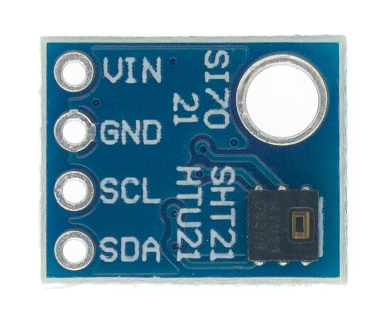
\includegraphics[width=.2\textwidth]{./Figures/sensor_htu21.png}
    \caption{Sensor HTU21.}
    \label{fig:htu21}
\end{figure}

\begin{itemize}
	\item Sensor BME280 \citep{sensor_bme280}: es un sensor ambiental que mide la presión atmosférica, la humedad y la temperatura. Se comunica a través de I2C o SPI. Figura \ref{fig:bme280}.
\end{itemize}

\begin{figure}[H]
    \centering
    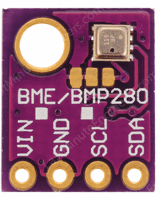
\includegraphics[width=.2\textwidth]{./Figures/sensor_bme280.png}
    \caption{Sensor BME280.}
    \label{fig:bme280}
\end{figure}

\begin{itemize}
	\item Sensor MH-Z19 \citep{sensor_mhz19}: es un sensor de dióxido de carbono basado en tecnología infrarroja no dispersiva (NDIR). La información se puede obtener a través de las interfaces UART o PWM. Figura \ref{fig:mhz19}.
\end{itemize}

\begin{figure}[H]
    \centering
    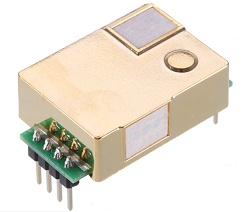
\includegraphics[width=.3\textwidth]{./Figures/sensor_mhz19.png}
    \caption{Sensor MH-Z19.}
    \label{fig:mhz19}
\end{figure}


%----------------------------------------------------------------------------------------
\section{Tecnologías de firmware}

En esta sección se presenta la tecnología utilizada en el trabajo, explicando qué es y las razones de su elección.

\subsection{MicroPython}

MicroPython es una versión reducida y optimizada de Python 3, escrita en C, diseñada para ejecutarse en microcontroladores con recursos limitados (como la memoria y  la capacidad de procesamiento). A diferencia de otros lenguajes de programación, MicroPython es interpretado, lo que significa que el código no se compila previamente, sino que se interpreta durante la ejecución.

Cuenta con un compilador cruzado, que convierte scripts de Python en bytecode que puede ser ejecutado eficientemente en hardware. Ofrece una biblioteca estándar adaptada a entornos limitados, lo que permite a los desarrolladores escribir código de alto nivel sin recurrir a lenguajes más complejos como C o ensamblador.

Al ser de código abierto, MicroPython está disponible para ser usado y modificado por cualquier persona. Este enfoque abierto, junto con su capacidad de funcionar en hardware limitado, lo hace ideal para la creación de aplicaciones embebidas \citep{micropython} \citep{infoMpy}. 

\subsubsection{Elección de MicroPython}
MicroPython fue elegido para este trabajo debido a varias ventajas clave:

\begin{itemize}
    \item Desarrollo ágil: al ser una versión optimizada de Python, permite un desarrollo rápido y eficiente, lo que es esencial para iterar y ajustar la funcionalidad del sistema y agregar nuevas características sin demoras.
    \item Pruebas y depuración sencillas: la capacidad de ejecutar scripts interactivos facilita la detección y corrección de errores en tiempo real, lo que acelera el proceso de desarrollo y depuración.
    \item Facilidad de integración con IoT: el ecosistema de MicroPython incluye bibliotecas que permiten integrar fácilmente protocolos de comunicación como ESP-NOW y MQTT, esenciales para la transmisión de datos  desde los sensores al gateway y de este al servidor IoT.
    \item Soporte y comunidad activa: cuenta con una amplia comunidad y documentación \citep{docsmpy}.
\end{itemize}

%----------------------------------------------------------------------------------------
\section{Protocolos de comunicación}

En esta sección se presentan los protocolos utilizados en el trabajo.

\subsection{Protocolo ESP-NOW}

ESP-NOW es un protocolo de comunicación inalámbrica desarrollado por Espressif para sus dispositivos. A diferencia de los protocolos convencionales que operan en varias capas del modelo OSI, ESP-NOW se basa exclusivamente en la capa de enlace de datos (capa 2), lo que simplifica la comunicación al reducir las cinco capas del modelo OSI a una sola, esto se puede observar en la figura \ref{fig:espnow}. Esta arquitectura optimizada le permite ser extremadamente eficiente en términos de recursos, ya que ocupa menos CPU y memoria flash en los dispositivos, crucial para aplicaciones IoT con restricciones de energía y recursos \citep{espnow}.

\begin{figure}[H]
    \centering
    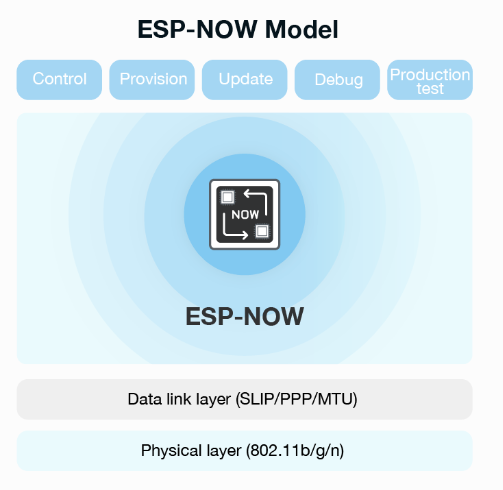
\includegraphics[width=.6\textwidth]{./Figures/espnow.png}
    \caption{Modelo ESP-NOW.}
    \label{fig:espnow}
\end{figure}

ESP-NOW permite la transmisión directa de datos entre dispositivos sin necesidad de una red Wi-Fi o internet. Además, puede funcionar junto con Wi-Fi y Bluetooth LE, y así ofrecer flexibilidad para integrarse en sistemas híbridos.

El protocolo admite transmisión \textit{unicast} y \textit{broadcast}, lo que facilita la comunicación eficiente entre múltiples dispositivos en redes distribuidas. También optimiza el consumo energético, lo que permite a los dispositivos operar en modo de baja potencia, esencial en nodos sensores que operan con baterías y donde la optimización de consumo es crítica.
Por último, ESP-NOW soporta encriptación, que garantiza la seguridad en la transmisión de datos entre los nodos \citep{espnowinfo}.

\subsection{Protocolo MQTT}

MQTT (\textit{Message Queuing Telemetry Transport}) es un protocolo de mensajería ligero y eficiente, diseñado para redes con ancho de banda limitado o donde se necesita una comunicación de baja latencia \citep{mqtt} \citep{mqttinfo}. 
Este se ejecuta sobre TCP/IP y utiliza una arquitectura de publicación/suscripción, donde:

\begin{itemize}
	\item \textit{Broker}: es el servidor central que recibe mensajes de los publicadores y los distribuye a los suscriptores. Gestiona todo el flujo de datos.
	\item Clientes: son dispositivos que actúan como publicadores (envían mensajes al \textit{broker}) o suscriptores (reciben mensajes según el tema suscrito).
	\item Temas: los mensajes se organizan por temas (\textit{topics}). Los publicadores envían datos asociados a un tema y los suscriptores reciben esos datos si están suscritos al tema correspondiente.
\end{itemize}

En la figura \ref{fig:arqmqtt} se puede observar la arquitectura del protocolo.

\begin{figure}[H]
    \centering
    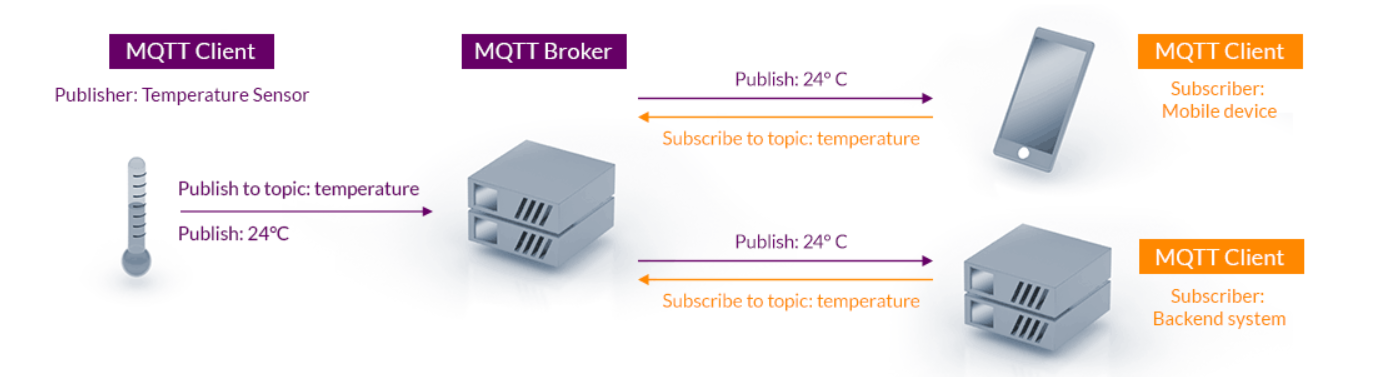
\includegraphics[width=1.1\textwidth]{./Figures/arq_mqtt.png}
    \caption{Arquitectura MQTT \citep{mqtt}.}
    \label{fig:arqmqtt}
\end{figure}

Algunas características claves del protocolo son: 

\begin{itemize}
	\item Retención de mensajes: el \textit{broker} puede almacenar el último mensaje publicado en un tema, y enviarlo a nuevos suscriptores cuando se conectan.
	\item Calidad de Servicio (QoS): Ofrece tres niveles de garantía de entrega:
	\begin{itemize}
		\item QoS 0: el mensaje se entrega una sola vez, sin confirmación.
		\item QoS 1: el mensaje se entrega al menos una vez.
		\item QoS 2: el mensaje se entrega exactamente una vez.
	\end{itemize}
	\item Conexión persistente: mantiene la conexión abierta con TCP/IP.
	\item \textit{Last Will and Testament} (LWT): notifica al \textit{broker} si un cliente se desconecta inesperadamente.
\end{itemize}


%----------------------------------------------------------------------------------------
\section{Aplicación web progresiva}

Una Aplicación Web Progresiva (PWA) es una aplicación web que utiliza tecnologías avanzadas para ofrecer una experiencia similar a la de una aplicación nativa en dispositivos móviles o de escritorio. Aunque se accede a través de un navegador, las PWA pueden instalarse en el dispositivo y ejecutarse como si fueran aplicaciones normales, sin necesidad de descargarlas desde una tienda de aplicaciones.
Las PWA combinan las mejores características de las aplicaciones web (accesibilidad desde cualquier navegador y plataforma) con las ventajas de las aplicaciones nativas (rendimiento rápido, funcionamiento sin conexión y capacidad de enviar notificaciones) \citep{pwamicrosoft} \citep{pwamozilla}.

Algunas ventajas clave de las PWA son \citep{pwaiebschool}:

\begin{itemize}
	\item Multiplataforma: funcionan en cualquier dispositivo con un navegador, sin necesidad de adaptar el código a diferentes sistemas operativos.
	\item Instalable: se puede agregar directamente desde el navegador, lo que facilita el proceso para el usuario.
	\item Funciona sin conexión: utilizan tecnologías como los \textit{Service Workers} \citep{serviceworker}, que permiten que la aplicación funcione incluso sin conexión a internet, permitiendo el acceso a datos almacenados previamente.
	\item Notificaciones: las PWA pueden enviar notificaciones al dispositivo, para mantener al usuario informado e interactuar con la aplicación, similar a las aplicaciones nativas.
	\item Menor consumo de almacenamiento: al no requerir una instalación completa como una aplicación nativa, ocupan menos espacio en el dispositivo.
	\item Menor costo de desarrollo y mantenimiento: se desarrollan utilizando tecnologías web estándar (HTML, CSS, JavaScript), por lo que no es necesario crear versiones separadas para diferentes sistemas operativos (Android, iOS).
\end{itemize}


%----------------------------------------------------------------------------------------
\section{Servidor de internet de las cosas}

En esta sección se describe qué es un servidor IoT y OpenRemote.

\subsection{Servidor IoT}
Un servidor IoT (\textit{Internet of Things}) es una plataforma o sistema que permite la gestión, almacenamiento y procesamiento de datos generados por dispositivos IoT conectados a una red. Estos dispositivos pueden ser sensores, actuadores, cámaras, entre otros, que recopilan información en tiempo real y la envían al servidor para su análisis o toma de decisiones.

\subsection{OpenRemote}

OpenRemote \citep{openremote} \citep{docsopenremote} es una plataforma de código abierto para gestionar y controlar redes de dispositivos IoT y sistemas conectados. Facilita la automatización y el manejo de datos en aplicaciones como ciudades inteligentes, edificios automatizados, monitoreo ambiental y gestión de energía.

Características principales de OpenRemote:

\begin{itemize}
	\item Gestión de dispositivos: permite conectar y controlar dispositivos IoT de diferentes tipos, independientemente del fabricante o del protocolo que utilicen.
	\item Panel de control personalizable: los usuarios pueden crear interfaces gráficas personalizadas para monitorear y controlar dispositivos en tiempo real.
	\item Procesamiento de datos: recibe datos de los dispositivos IoT y los procesa, para generar informes, alertas o acciones automatizadas basadas en reglas predefinidas.
	\item Protocolos de comunicación: soporta una amplia variedad de protocolos de IoT como MQTT, HTTP, entre otros.
	\item Automatización y reglas: los usuarios pueden definir reglas y flujos de trabajo para automatizar respuestas o acciones en función de los datos recibidos.
\end{itemize}

En la figura \ref{fig:arqopremote} se puede observar la arquitectura general del servidor.

\begin{figure}[H]
    \centering
    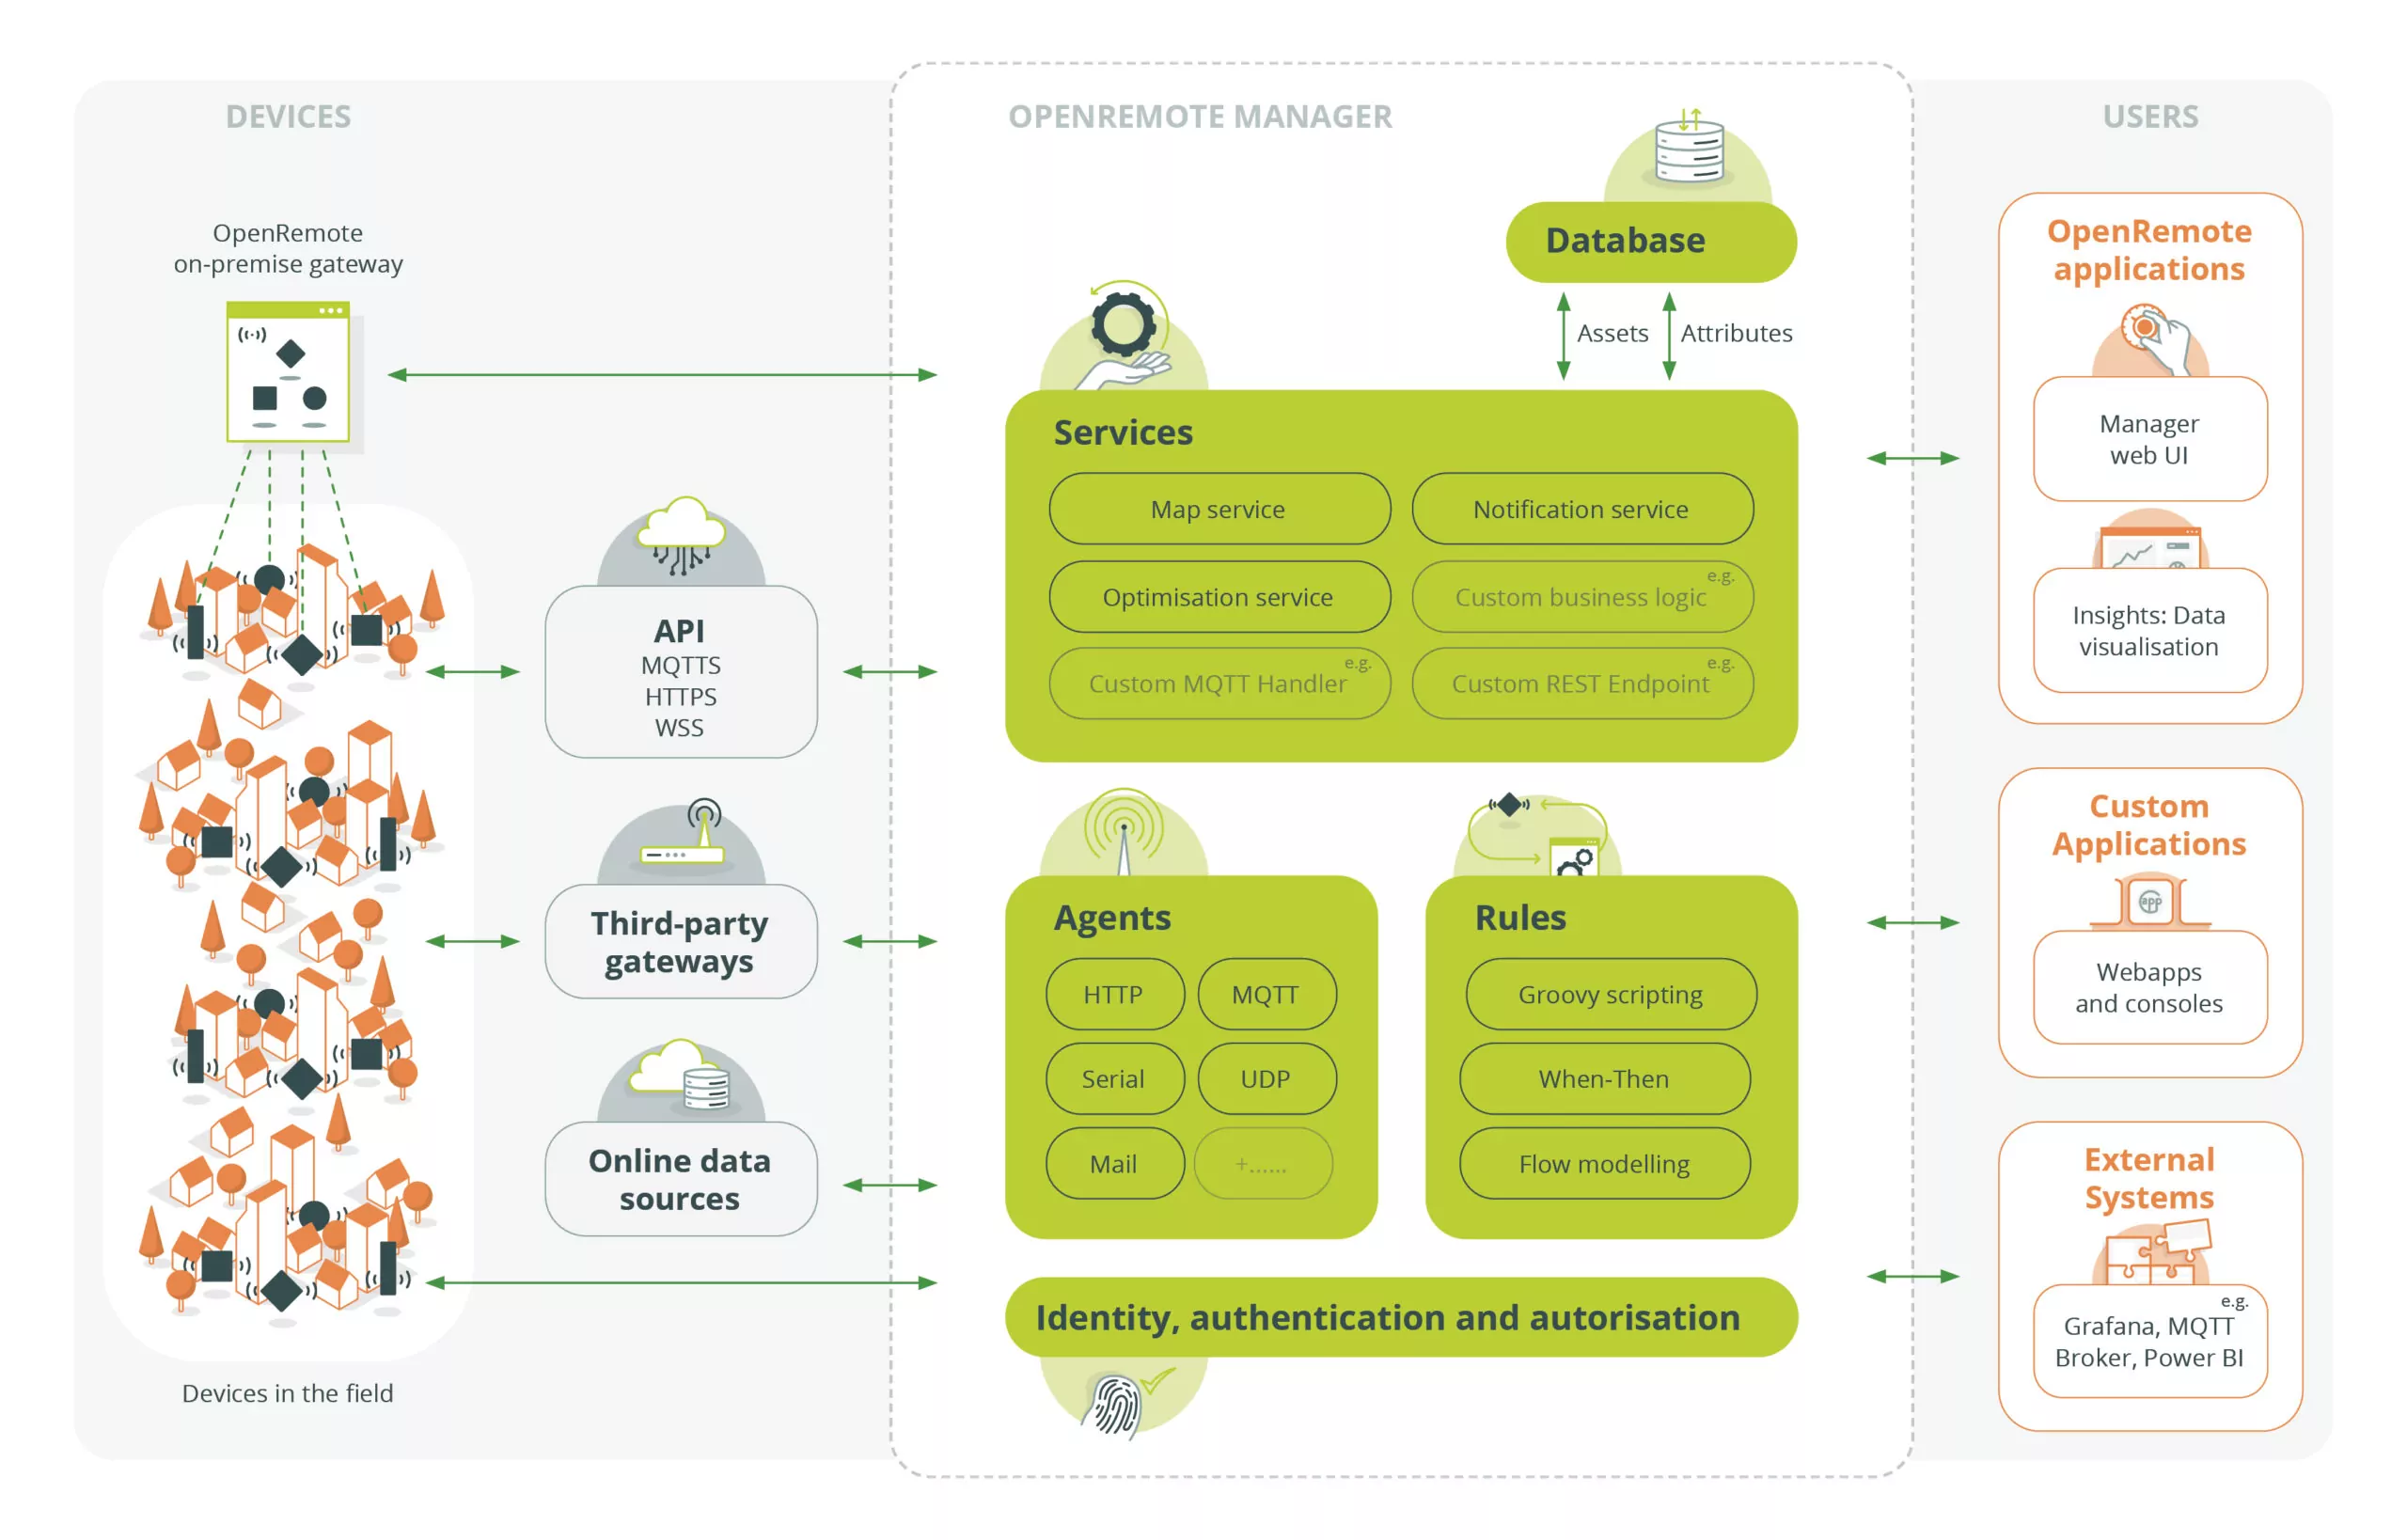
\includegraphics[width=1.2\textwidth]{./Figures/arq_or.jpg}
    \caption{Arquitectura OpenRemote \citep{docsopenremote}.}
    \label{fig:arqopremote}
\end{figure}


%----------------------------------------------------------------------------------------



